\section{Core}

% The core of Brel consists of filings, facts, components and QNames, where each element is represented by one or more classes.
% In essence, each filing consists of a set of facts and components. 
% QNames are used all across Brel, which is why they are considered part of the core.
% The following UML diagram shows the core of Brel.
The foundation of Brel is built upon filings, facts, components, and QNames, where each component is encapsulated within one or more classes.
At its core, every filing is comprised of numerous facts and components.
QNames are extensively employed throughout Brel, highlighting their importance as a core element.
The UML diagram provided below illustrates the core components of Brel.

\begin{figure}[H]
    \centering
    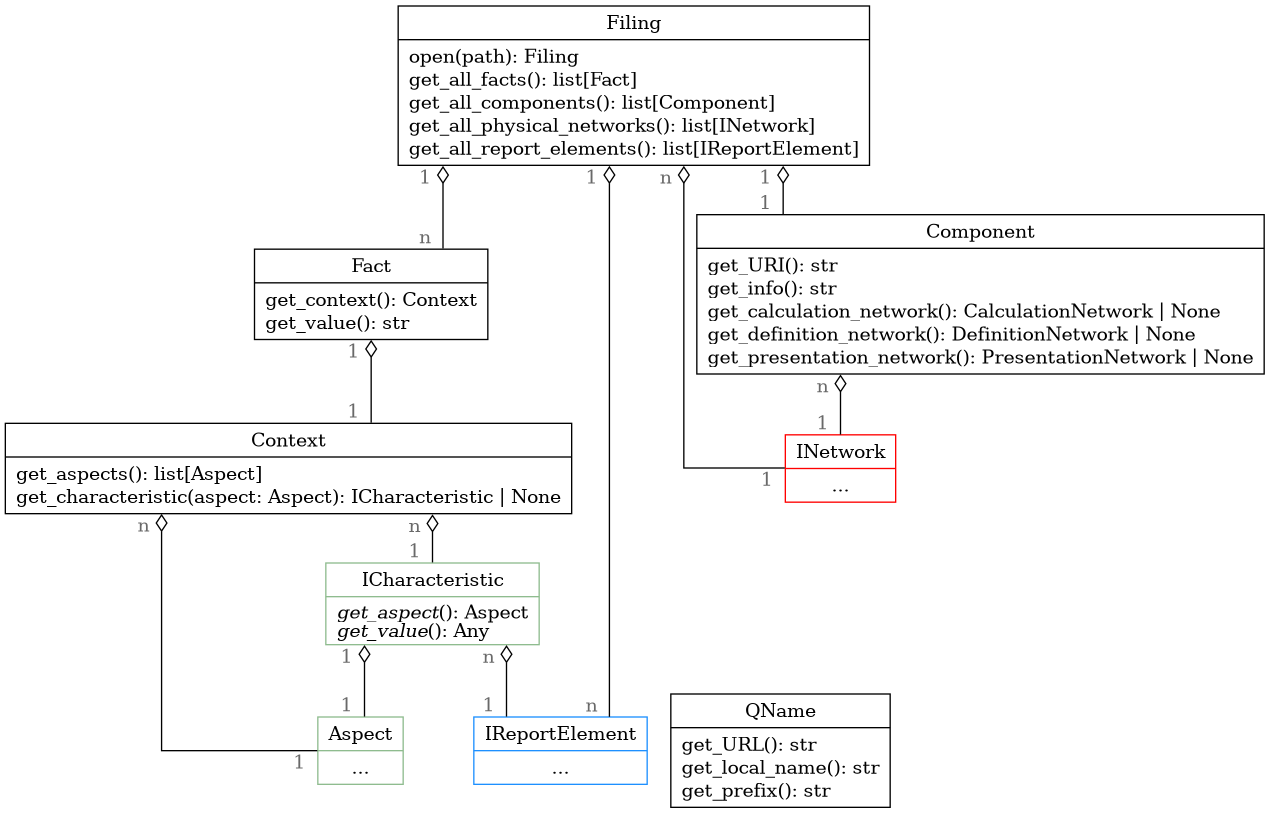
\includegraphics[width=\textwidth]{images/brel_core_classes.png}
    \caption{UML diagram of the core of Brel}
    \label{fig:brel_core_classes}
\end{figure}

\subsection{Filing}
\label{subsec:filing}

% Starting with the \texttt{Filing} class, it represents a single XBRL filing.
% Obviously, it needs a method for loading a filing from a file, directory, or URL.
% The \texttt{Filing.open} covers all of these cases. 
% It takes a single argument, which can be a file path, directory path or URL.
% The method will automatically detect the type of the argument and load the filing accordingly.
% It will also reject any invalid arguments.
The \texttt{Filing} class is designed to represent an individual XBRL filing.
A key functionality of this class is the \texttt{Filing.open} method, which facilitates the loading of a filing from various sources such as a file, directory, or URL.
This method accepts a single parameter that could be a path to a file or directory, or a URL, and intelligently determines the type of input to process the filing.
It also ensures the rejection of any inputs that are not valid.

% The next two methods are \texttt{Filing.get\_all\_facts} and \texttt{Filing.get\_all\_components},
% which return all facts and components of the filing, respectively.
% Both the facts and components are returned as a list of \texttt{Fact} and \texttt{Component} objects.
% The order of the facts and components is not guaranteed.
% Brel does provide helper methods for getting specific facts and components,
% but their functionality can be easily implemented using the \texttt{get\_all\_facts} and \texttt{get\_all\_components} methods.
Following this, the methods \texttt{Filing.get\_all\_facts} and \texttt{Filing.get\_all\_components} are available to retrieve all facts and components of a filing, respectively.
These are returned as lists of \texttt{Fact} and \texttt{Component} objects, though the order of the facts and components is arbitrary.
While Brel offers helper methods for accessing specific facts and components, the aforementioned methods can be used to achieve similar outcomes.

% There exist some networks that are not part of any Component, specifically \texttt{physical\ networks}.
% These networks cannot be accessed indirectly through Components, 
% which is why the \texttt{Filing} class also provides a method for getting all physical networks.
% This method is aptly named \texttt{Filing.get\_all\_physical\_networks}.
Moreover, there are certain networks, termed \texttt{physical networks}, which do not belong to any Component.
Direct access to these networks through Components is not possible, 
hence the \texttt{Filing} class provides a \texttt{Filing.get\_all\_physical\_networks} method for retrieving all physical networks.

% Similar to networks that are not part of any Component, 
% there are also report elements that are not part of any network or fact.
% The method \texttt{Filing.get\_all\_report\_elements} returns all report elements of the filing,
% including both report elements that are referenced by facts or networks and those that are not.
Additionally, the \texttt{Filing} class caters to report elements that are neither associated with any network nor fact.
The \texttt{Filing.get\_all\_report\_elements} method returns all such report elements within a filing, 
% encompassing those linked to facts or networks and those without any association.
including those not referenced by facts or networks.

% The two most important classes associated with a filing are \texttt{Fact} and \texttt{Component}.
% Both classes encompass two different core aspects of XBRL.
% All classes belonging to facts are covered by the Open Information Model (OIM)\cite{oim}.
% Their design will therefore answer research question \ref{itm:research_question_1}.
% Classes belonging to components mostly involve topics that are not covered by the OIM.
% Consequently, their design will answer research question \ref{itm:research_question_2}.
The essential classes tied to a filing are the \texttt{Fact} and \texttt{Component} classes, each addressing different fundamental aspects of XBRL.
The \texttt{Fact} class and its related classes are governed by the Open Information Model (OIM)\cite{oim}, addressing research question \ref{itm:research_question_1}.
Conversely, the \texttt{Component} class and its related entities delve into areas beyond the OIM's scope, thus addressing research question \ref{itm:research_question_2}.

% The subsequent sections will first describe the \texttt{QName} class,
% since it is used by numerous other classes.
% The next few sections will cover the \texttt{Fact} class and all of its associated classes.
% Finally, the last subsections are dedicated to the \texttt{Component} class and its associated classes.
The discussion will proceed with an examination of the \texttt{QName} class, given its utility across numerous other classes.
Subsequent sections will explore the \texttt{Fact} class along with its related classes.
The final segments will focus on the \texttt{Component} class and its associated classes.

% \subsection{QName}
% \label{subsec:qname}

% The \texttt{QName} class represents a qualified name, which is a combination of a namespace and a local name.
% It is the only remnant of the underlying XML structure of XBRL in the Brel API.
% Since it already provides an elegant way of identifying elements across different namespaces,
% We chose to keep it in the API.

% As described in chapter \ref{chapter:xbrl}, a QName is a combination of a namespace URL, a prefix and a local name.
% Naturally, the \texttt{QName} class provides methods for accessing all three of these components.
% These methods are fittingly named \texttt{QName.get\_URL}, \texttt{QName.get\_prefix} and \texttt{QName.get\_local\_name}.

\subsection{QName}
\label{subsec:qname}

The \texttt{QName} class signifies a qualified name, merging a namespace with a local name.  
This element is the singular link to XBRL's XML background found in the Brel API.  
Its effectiveness in identifying elements across various namespaces led to its inclusion in the API.  

As outlined in chapter \ref{chapter:xbrl}, a QName consists of a namespace URL, a prefix, and a local name.  
Therefore, the \texttt{QName} class provides methods to retrieve these components:  
\texttt{QName.get\_URL} for the namespace URL, \texttt{QName.get\_prefix} for the prefix, and \texttt{QName.get\_local\_name} for the local name.

\subsection{Fact}
\label{subsec:fact}

% The \texttt{Fact} class represents, as the name suggests, a single XBRL fact.
% When boiled down to its core, a fact consists of a value and a set of characteristics that describe what the value represents.
% The value of a fact is represented by the \texttt{Fact.get\_value} method, which returns the value as a string.
% The characteristics of a fact are represented by the \texttt{Fact.get\_context} method.
% A context is a set of characteristics that describe the fact.
% In other terms, each fact occupies a position in a multi-dimensional space, where each characteristic represents a point along one dimension.
The \texttt{Fact} class symbolizes a single XBRL fact, encapsulating a value along with various characteristics that give context to the value.
The method \texttt{Fact.get\_value} returns the value as a string.
Characteristics defining a fact are accessible through the \texttt{Fact.get\_context} method, which consists of a set of characteristics that describe the fact.
Essentially, each fact is situated within a multi-dimensional space, with each characteristic pinpointing one dimension's coordinate.

% One design decision that seems questionable at first is the \texttt{Fact.get\_value} method, which returns the value as a string.
% Not all values in XBRL are strings.
% Some are integers, decimals, dates, etc.
% The reason for this design decision is that Facts have a unit characteristic, which determines the type of the value.
% Therefore, units in XBRL are represented as a dimension of the fact's context.
% Since all values that XBRL facts can take are representable as strings, the \texttt{Fact.get\_value} method returns the value as a string,
% since it is the most general representation of the value.
At first glance, the choice to return fact values as strings via \texttt{Fact.get\_value} might raise questions, 
given that XBRL values encompass a range of types, including integers, decimals, dates, etc.
This approach stems from the understanding that facts possess a unit characteristic, which categorizes the value's type.
Units in XBRL thus act as a contextual dimension for a fact.
The string format for all values ensures a universal representation, considering strings can encapsulate any XBRL fact value.

% Brel does however provide helper methods for converting the value into the type that most appropriately represents the value.
% The helper method checks the unit of the fact and converts the value accordingly.
Nevertheless, Brel facilitates type-appropriate conversions of these values through helper methods.
These methods assess the fact's unit to convert the string value into a more suitable data type, aligning with the specific nature of the value.

\subsection{Context}

% Contexts, as described in section \ref{subsec:fact}, are sets of characteristics what a fact represents.
% The \texttt{Context} class represents a single context.
% Each fact has its own context and each context belongs to exactly one fact.
% \footnote{There might be multiple contexts that have identical characteristics, but they are still represented as separate objects.}
% Contexts provide two methods for accessing their characteristics.
% The \texttt{Context.get\_aspects} method returns a list of all aspects for which the context has a characteristic.
% The \texttt{Context.get\_characteristic} method returns the characteristic of the context for a given aspect.
% If the context does not have a characteristic for the given aspect, the method returns \texttt{None}.
Contexts, as outlined in section \ref{subsec:fact}, constitute sets of attributes that describe what a fact represents.
The \texttt{Context} class embodies an individual context, with each fact possessing a unique context, and every context being linked to a singular fact.
\footnote{Although there may be multiple contexts with the same characteristics, they are treated as distinct entities.}
Contexts offer two methods for characteristic retrieval.
The \texttt{Context.get\_aspects} method yields a list of all aspects associated with characteristics within the context.
For instance, most contexts in XBRL have the aspects entity, period, unit and concept.
% The \texttt{Context.get\_characteristic} method returns the specific characteristic of the context for a designated aspect, returning \texttt{None} if the context lacks a characteristic for that aspect.
Given an aspect, the \texttt{Context.get\_characteristic} method returns the corresponding characteristic.
For example, the unit aspect of a context might return the characteristic "USD".
The API of both Aspects and Characteristics will be covered in section \ref{sec:characteristics}.

% To reiterate, a characteristic represents a point along a dimension single dimension.
% Multiple characteristics can be combined to form a point in a multi-dimensional space.
To elaborate, a characteristic denotes a coordinate along a singular dimension, 
and aggregating multiple characteristics constructs a coordinate within a multi-dimensional framework.

One such point might be "Foo Inc.'s net income for the year 2020 in USD".\label{point:foo_net_income}
Another point might be "Bar Corp.'s net income for the year 2021 in CHF".
Each represents a position within a four-dimensional hypercube
\footnote{The dimensions in these instances are entity, period, unit, and concept.}.
% Both points point to values in a four-dimensional hypercube.
% \footnote{In these examples, the four dimensions are entity, period, unit and concept.}

% \subsection{Aspect and Characteristic}

% Aspects describe the dimensions along which characteristics are positioned.
% Their API is described in section \ref{sec:characteristics}, which will be covered in a later portion of this chapter.

\subsection{Report Elements}

% Report elements are the building blocks of XBRL filings.
% Probably the most important report element is the concept, initially explained in section \ref{sec:concepts}.
% In figure \ref{fig:brel_core_classes}, the interface \texttt{IReportElement} represents all report elements, not just concepts.
Report elements form the foundational aspects of XBRL filings, with concepts being among the most crucial, as initially discussed in section \ref{sec:concepts}.
In figure \ref{fig:brel_core_classes}, the \texttt{IReportElement} interface is depicted as representing all types of report elements, not solely concepts.

% Obviously, some characteristics use report elements to describe the position of a fact along a dimension.
% Take the previous example \ref{point:foo_net_income} for instance.
% One of the characteristics uses the concept "net income" to describe the position of the fact along the concept dimension.
% In this case, the characteristic is uses the concept "net income". 
Characteristics often utilize report elements to denote a fact's position within a dimension.
Referring back to the example in \ref{point:foo_net_income}, the "net income" concept is employed as a characteristic to define the fact's location along the concept dimension.

% Since there are multiple types of report elements, the \texttt{IReportElement} interface provides a method for getting the type of the report element.
% Report elements have their own dedicated section \ref{sec:report_elements}, which will be covered in a later portion of this chapter.

% Given the variety of report elements, the \texttt{IReportElement} interface includes a method to ascertain the type of the report element.
% A more detailed discussion on report elements is scheduled in section \ref{sec:report_elements}, to be addressed later in this chapter.
Given the diversity of report elements, the \texttt{IReportElement} interface includes a method for getting the type of the report element.
A more detailed discussion on report elements is scheduled in section \ref{sec:api_report_elements}, to be addressed later in this chapter.

\subsection{Component}

% Moving on to the other side of figure \ref{fig:brel_core_classes}, the \texttt{Component} class represents the chapters of a filing.
% Components are the first class not by the OIM.

% Each component consists of a number of networks and an identifier.
% A component can have at most one network of each type.
% The available network types are calculation-, presentation- and definition networks.
% Additionally, a component can have an optional human-readable description of what the component represents.
Transitioning to the \texttt{Component} class, as illustrated on the opposite end of figure \ref{fig:brel_core_classes}, 
it symbolizes the chapters within a filing and represents a structure not covered by the OIM.

Each component is characterized by a series of networks and an identifier.
Components can contain no more than one network of each type.
The types of networks include calculation, presentation, and definition networks.
A component may also feature an optional, human-readable description elucidating its purpose.

% The \texttt{Component.get\_calculation\_network}, \texttt{Component.get\_presentation\_network} and \texttt{Component.get\_definition\_network} methods
% return the calculation, presentation and definition network of the component, respectively.
% Each of these methods can return \texttt{None}, if the component does not have a network of the requested type.
The methods \texttt{Component.get\_calculation\_network}, \texttt{Component.get\_presentation\_network}, 
and \texttt{Component.get\_definition\_network} respectively retrieve the component's calculation, presentation, and definition networks.
Each method may return \texttt{None} if the component lacks a network of the specified type.

% The \texttt{Component.get\_uri} method returns the identifier of the component,
% which is a URI that uniquely identifies the component within the filing.

% The \texttt{Component.get\_info} method returns the human-readable description of the component, if it exists.
% If the component does not have a description, the method returns an empty string.
The \texttt{Component.get\_uri} method yields the component's identifier, a URI that distinctively identifies the component within the filing.

Moreover, \texttt{Component.get\_info} delivers the component's human-readable description when available, or an empty string if absent.

% The networks that are part of a component are represented by the \texttt{Network} class.
% Networks will be covered in the second half of this chapter.
% The first half focuses on OIM concepts, while the second half focuses on non-OIM concepts.
The networks within a component implement the \texttt{INetwork} interface, set to be discussed in the latter half of this chapter.
